\documentclass[tikz,border=2pt]{standalone}
\usepackage{amsmath,amssymb}
\usepackage{tikz}
\usetikzlibrary{arrows.meta}

\begin{document}
% A subspace must contain 0 and be closed under + and scaling: a plane through the origin
% qualifies, a shifted plane does not.
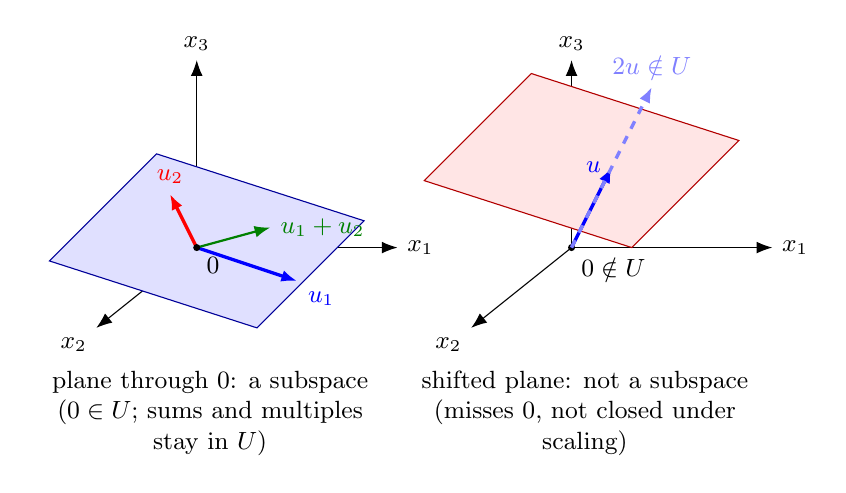
\begin{tikzpicture}[scale=0.85, every node/.style={font=\small}, >={Latex[length=2mm]}]
	\begin{scope}
		\draw[->] (0,0) -- (3.0,0) node[right] {$x_1$};
		\draw[->] (0,0) -- (0,2.8) node[above] {$x_3$};
		\draw[->] (0,0) -- (-1.5,-1.2) node[below left] {$x_2$};
		\fill[blue!12] (-2.2,-0.2) -- (0.9,-1.2) -- (2.5,0.4) -- (-0.6,1.4) -- cycle;
		\draw[blue!60!black] (-2.2,-0.2) -- (0.9,-1.2) -- (2.5,0.4) -- (-0.6,1.4) -- cycle;
		\draw[->, blue, very thick] (0,0) -- (1.5,-0.5) node[below right] {$u_1$};
		\draw[->, red, very thick] (0,0) -- (-0.4,0.8) node[above] {$u_2$};
		\draw[->, green!50!black, thick] (0,0) -- (1.1,0.3) node[right] {$u_1+u_2$};
		\fill (0,0) circle (1.5pt) node[below right] {$0$};
		\node[anchor=north, align=flush center, text width=4.4cm] at (0.2,-1.7) {plane through $0$: a subspace ($0\in U$; sums and multiples stay in $U$)};
	\end{scope}
	\begin{scope}[xshift=5.6cm]
		\draw[->] (0,0) -- (3.0,0) node[right] {$x_1$};
		\draw[->] (0,0) -- (0,2.8) node[above] {$x_3$};
		\draw[->] (0,0) -- (-1.5,-1.2) node[below left] {$x_2$};
		\fill[red!10] (-2.2,1.0) -- (0.9,0.0) -- (2.5,1.6) -- (-0.6,2.6) -- cycle;
		\draw[red!70!black] (-2.2,1.0) -- (0.9,0.0) -- (2.5,1.6) -- (-0.6,2.6) -- cycle;
		\fill (0,0) circle (1.5pt) node[below right] {$0\notin U$};
		\draw[->, blue, very thick] (0,0) -- (0.6,1.2) node[left] {$u$};
		\draw[->, blue!50, very thick, dashed] (0,0) -- (1.2,2.4) node[above] {$2u\notin U$};
		\node[anchor=north, align=flush center, text width=4.4cm] at (0.2,-1.7) {shifted plane: not a subspace (misses $0$, not closed under scaling)};
	\end{scope}
\end{tikzpicture}
\end{document}
